\documentclass[a4paper]{arrowhead}

\usepackage[yyyymmdd]{datetime}
\usepackage{etoolbox}
\usepackage[utf8]{inputenc}
\usepackage{multirow}

\renewcommand{\dateseparator}{-}

%% Special references
\newcommand{\scref}[2]{{\textcolor{ArrowheadBlue}{\hyperref[sec:services:consumed:#1]{#2}}}}
\newcommand{\scdef}[2]{{\textcolor{ArrowheadBlue}{#2\label{sec:services:consumed:#1}}}}
\newcommand{\spref}[2]{{\textcolor{ArrowheadBlue}{\hyperref[sec:services:produced:#1]{#2}}}}
\newcommand{\spdef}[2]{{\textcolor{ArrowheadBlue}{#2\label{sec:services:produced:#1}}}}
%%

\begin{document}

%% Arrowhead Document Properties
\ArrowheadTitle{Authorization}
\ArrowheadType{System Design Description}
\ArrowheadTypeShort{SysDD}
\ArrowheadVersion{4.3.0}
\ArrowheadDate{\today}
\ArrowheadAuthor{Szvetlin Tanyi}
\ArrowheadStatus{RELEASE}
\ArrowheadContact{szvetlin@aitia.ai}
\ArrowheadFooter{\href{www.arrowhead.eu}{www.arrowhead.eu}}
\ArrowheadSetup
%%

%% Front Page
\begin{center}
  \vspace*{1cm}
  \huge{\arrowtitle}

  \vspace*{0.2cm}
  \LARGE{\arrowtype}
  \vspace*{1cm}
  \vspace*{\fill}

  % Front Page Image
  %\includegraphics{figures/TODO}

  \vspace*{1cm}
  \vspace*{\fill}

  % Front Page Abstract
  \begin{abstract}
    This document describes the Authorization core system of the Eclipse Arrowhead Framework. This core system takes responsibility for managing the offered services of all systems.
  \end{abstract}

  \vspace*{1cm}

  \scriptsize
  \begin{tabularx}{\textwidth}{l X}
    \raisebox{-0.5\height}{
\includegraphics[width=2cm]{figures/artemis_logo}} & {ARTEMIS Innovation Pilot Project: Arrowhead\newline
    THEME [SP1-JTI-ARTEMIS-2012-AIPP4 SP1-JTI-ARTEMIS-2012-AIPP6]\newline
    [Production and Energy System Automation Intelligent-Built environment and urban infrastructure for sustainable and friendly cities]}
  \end{tabularx}
  \vspace*{-0.2cm}
\end{center}
\newpage
%%

%% Table of Contents
\tableofcontents
\newpage
%%

\section{Overview}
\label{sec:overview}

This document describes the Eclipse Arrowhead  Authorization system,
which exists to manage and to authorize connection between various systems using Authorization Rules in a Eclipse Arrowhead Local Cloud (LC).  Examples of such interactions is a consumer system is allowed to consume some kind of Eclipse Arrowhead service offered by an other systems in the LC, because a previously set Authorization Rule enables it. 

This Core System provides a database, which stores information related to the currently actively enforced Authorization Rules  within the Local Cloud.

The purpose of this System is therefore to allow:
\begin{itemize}

\item Provide AuthorizationControl Service (both intra- and inter-Cloud).
\item Provide a TokenGeneration Service for allowing session control within the Local Cloud.
\end{itemize}

The purpose of the TokenGeneration functionality is to create session control functionality through the Core Sytems. The output is JSON Web Token that validates the Service Consumer system when it will try to access the Service from another Application System (Service Provider). This Token shall be primarily generated during the orchestration process and only released to the Service Consumer when all affected Core Systems are notified and agreed to the to-be-established Service connection.

This System (in line with all core Systems) utilizes the X.509 certificate Common Name naming convention in order to work.

The v4.3.0 only supports the HTTP protocol, JSON encoding and TLS payload protection. 


\section{System Role}
\label{sec:role}

This System only provides two Core Service the \textbf{AuthorizationControl} and \textbf{TokenGeneration}. 


There are two use case scenarios connected to the Service Registry.
\begin{itemize}
    \item Check access rights (invoke the AuthorizationControl).
    \item Generate an access token (the Orchestrator invokes the TokenGeneration).
\end{itemize}

\begin{figure}[t!]
  \centering 
  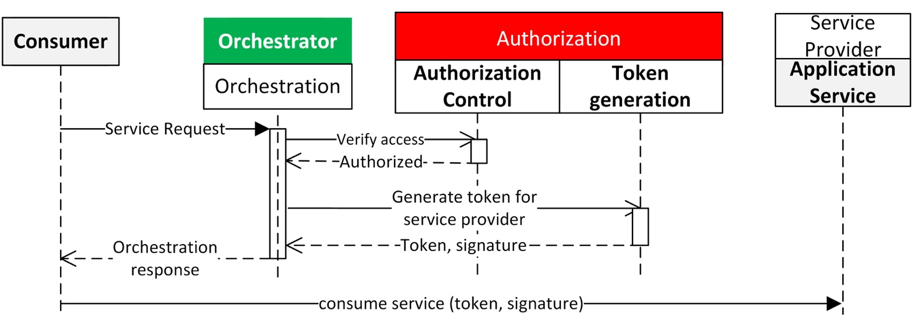
\includegraphics[width=0.8\textwidth]{figures/authorization_crosscheck.png}
  \caption{Authorization crosscheck during orchestration process. v4.3.0 only support HTTP/JSON/TLS.}
  \label{fig:ServiceRegistrySysDD}
\end{figure}

The AuthorizationControl Service provides 2 different interfaces to look up authorization rights:

\begin{itemize}
    \item Intra-Cloud authorization: defines an authorization right between a consumer and provider system in the same Local Cloud for a specific Service.
    \item Inter-Cloud authorization: defines an authorization right for an external Cloud to consume a specific Service from the Local Cloud.
\end{itemize}

\section{Services}
\label{sec:services}


\subsection{Consumed Services}

\subsubsection{\spdef{ServiceDiscovery}{ServiceDiscovery}}

This service is provided to allow other systems to \textbf{Register}
and to \textbf{Unregister} their services, and to \textbf{Query}
public services. In addition the service can Echo that its alive.

\subsection{Provided Services}

\subsubsection{\spdef{AuthorizationControl}{AuthorizationControl}}

This service is provided to allow the Orchestrator to check whether the requester is allowed to access the requested service. 

\subsubsection{\spdef{TokenGeneration}{TokenGeneration}}

This service is provided to allow access token generation for a consumer system.

\section{Security}
\label{sec:security}

This System can be secured via the HTTPS protocol. If it is started in secure mode, it verifies whether the Application System possesses a proper X.509 identity certificate and whether that certificate is Arrowhead compliant in its' making. This certificate structure and creation guidelines ensure:

\begin{itemize}
    \item Application System is properly bootstrapped into the Local Cloud
    \item The Application System indeed belongs to this Local Cloud
    \item The Application System then automatically has the right to register its Services in the Registry.
   
\end{itemize}

 If these criteria are met, the Application System’s registration or removal message is processed. An Application System can only delete or alter entries that contain the Application System as the Service Provider in the entry.



\newpage

\bibliographystyle{IEEEtran}
\bibliography{bibliography}

\newpage

\section{Revision History}
\subsection{Amendments}

\noindent\begin{tabularx}{\textwidth}{| p{1cm} | p{3cm} | p{2cm} | X | p{4cm} |} \hline
\rowcolor{gray!33} No. & Date & Version & Subject of Amendments & Author \\ \hline

1 & 2020-12-05 & 4.3.0 &  & Tanyi Szvetlin \\ \hline


\end{tabularx}

\subsection{Quality Assurance}

\noindent\begin{tabularx}{\textwidth}{| p{1cm} | p{3cm} | p{2cm} | X |} \hline
\rowcolor{gray!33} No. & Date & Version & Approved by \\ \hline

1 & 2021-01-26  & 4.3.0 & Jerker Delsing\\ \hline


\end{tabularx}

\end{document}